\documentclass[a4paper]{article}
\usepackage{graphicx} % Extended graphics inclusions
\usepackage{float}
\usepackage{url} % For \url{}
\usepackage{../config/atxy} % For front cover
\usepackage{amsfonts} % Needed for some fonts
\usepackage[usenames]{color} % Needed for colored R input/output
\usepackage{pdfcolmk} % Correct some problems with the color stack


\title{Cover}
\author{Humblot, L. \and Lobry, J.R.}

\usepackage{Sweave}
\begin{document}
%
% To change the R input/output style:
%
\definecolor{Soutput}{rgb}{0,0,0.56}
\definecolor{Sinput}{rgb}{0.56,0,0}
\DefineVerbatimEnvironment{Sinput}{Verbatim}
{formatcom={\color{Sinput}},fontsize=\footnotesize, baselinestretch=0.75}
\DefineVerbatimEnvironment{Soutput}{Verbatim}
{formatcom={\color{Soutput}},fontsize=\footnotesize, baselinestretch=0.75}
%
% This removes the extra spacing after code and output chunks in Sweave,
% but keeps the spacing around the whole block.
%
\fvset{listparameters={\setlength{\topsep}{0pt}}}
\renewenvironment{Schunk}{\vspace{\topsep}}{\vspace{\topsep}}
%
% Rlogo
%
\newcommand{\Rlogo}{\protect
\includegraphics[height=1.8ex,keepaspectratio]{../figs/Rlogo.pdf}}
%
% Shortcut for seqinR:
%
\newcommand{\seqinr}{\texttt{seqin\bf{R}}}
\newcommand{\Seqinr}{\texttt{Seqin\bf{R}}}
\fvset{fontsize= \scriptsize}
%
% R output options and libraries to be loaded.
%
%
%  Sweave Options
%
% Put all figures in the fig folder and start the name with current file name.
% Do not produce EPS files
%


\maketitle
\newpage
% BEGIN - DO NOT REMOVE THIS LINE

\thispagestyle{empty}
\atxy(0cm,0cm) {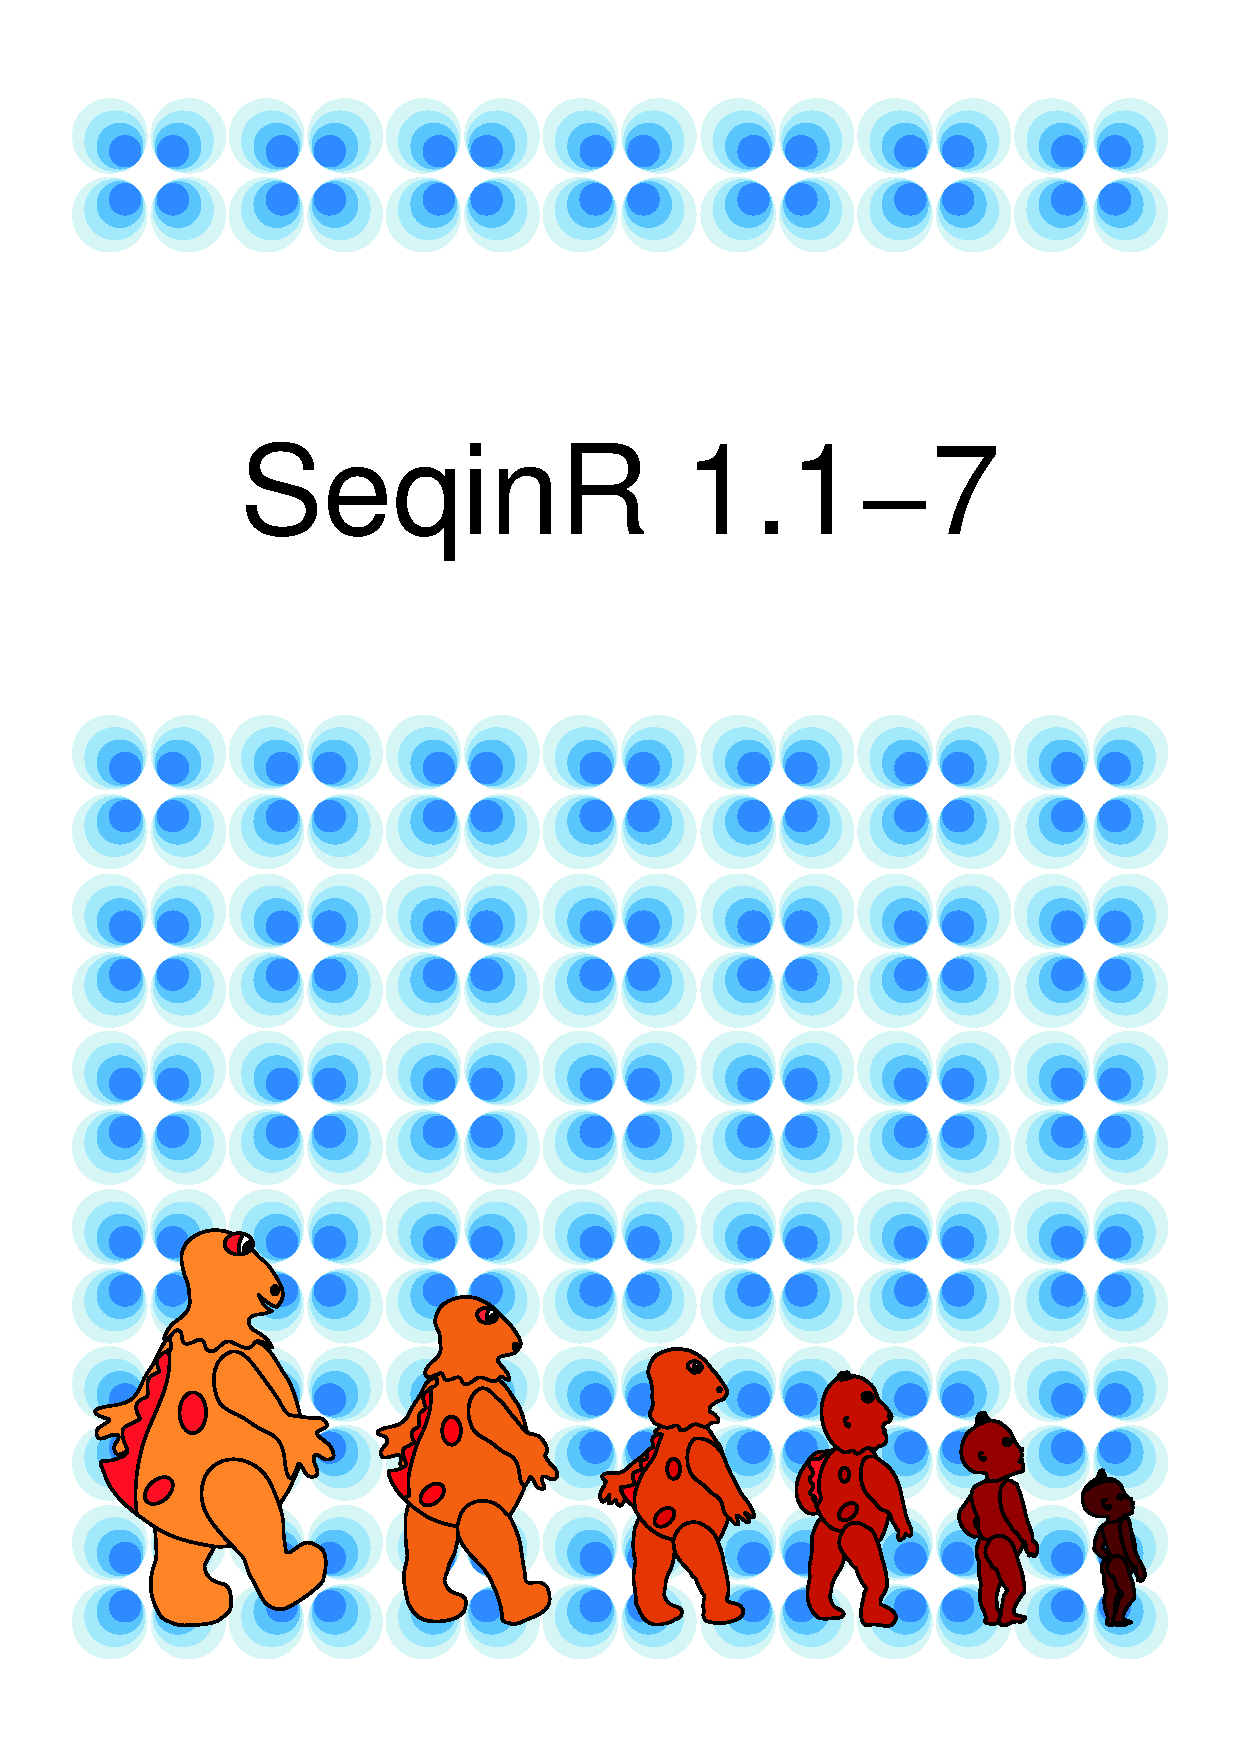
\includegraphics[width=\paperwidth,height=\paperheight]{../figs/cover}}
\clearpage
\newpage

\section*{The march of progress icon}

The cover, an artwork created\footnote{
with Canvas from  ACD Systems.}
by Lionel Humblot, is an allusion to what
Stephen J. Gould considered as a caonical icon of "[t]he most serious 
and pervasive of all misconceptions about evolution equates the 
concept with some notion of progress, usually inherent and predictable, 
and leading to a human pinnacle" \cite{GouldSJ1995}. Some examples
of the so-called "march of progress icon" out of hundreds in S.J. 
Gould's collection from popular press are given in the begining of his 
famous book \textit{Wonderful life} \cite{GouldSJ1989}.

\begin{figure}
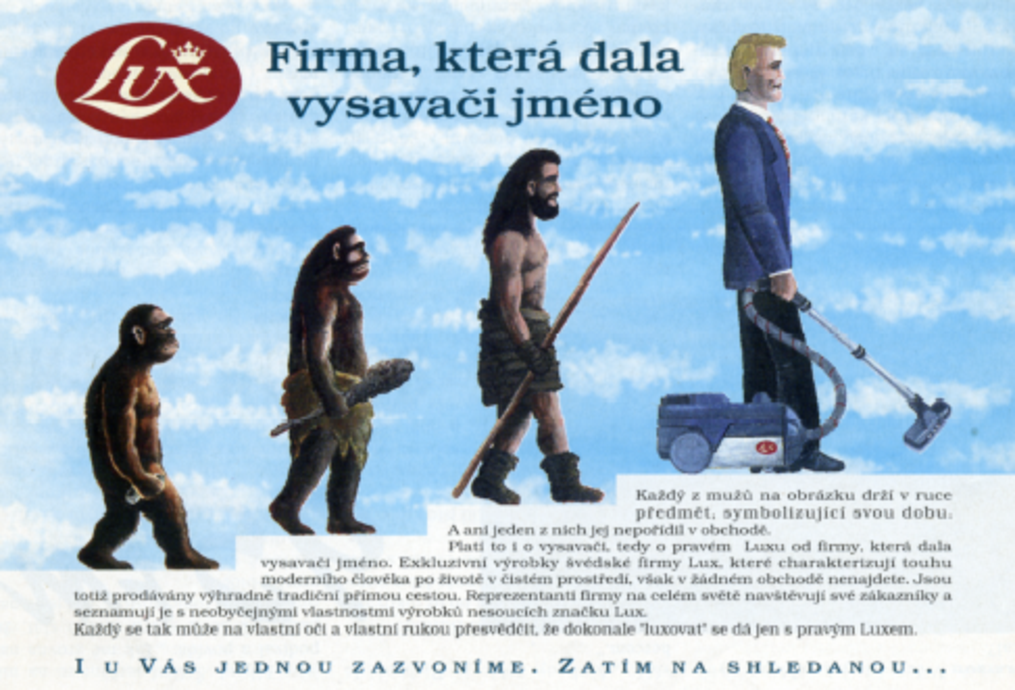
\includegraphics[width=\textwidth]{../figs/mop}
\caption{The march of progress icon is very common in popular press. This
example is from page 46 of a 1984 summer issue of the tchek edition 
of \textit{Playboy}.}
\label{mop}
\end{figure}

Note that the underlying conception predates Darwin \cite{LovejoyAO1936}.
We know now that evolution doesn not equal progress, and this is illutrated
here in the cover by the unusual \textbf{decreasing} size from the initial 
character (on the left) to the last one (on the right).

\section*{The character on the left}

The character on the left is called Casimir, the cult character of the french
TV show \textit{l'{\^i}le aux enfants}\marginpar{
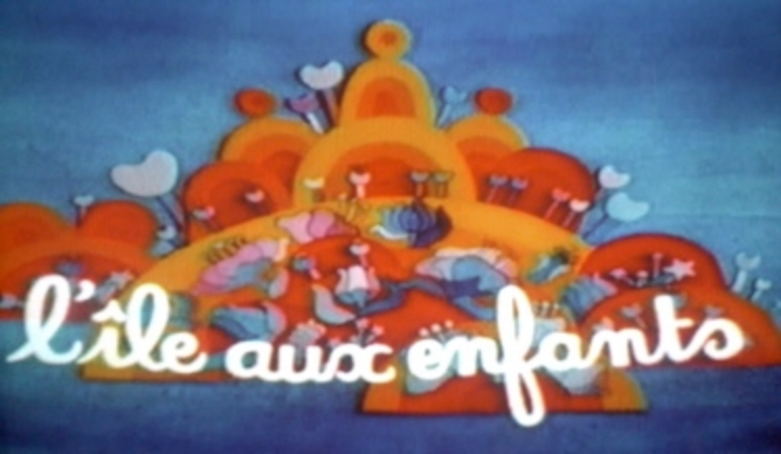
\includegraphics[width=\marginparwidth]{../figs/kidsisland}
\scriptsize{\textit{L'{\^i}le aux enfants}.}
} (literally Kid's island, a french adaptation
of \textit{Sesame Street} from 1974 to 1975 and then an autonomous
production until 1982 when it eventually ended). Casimir was a muppet, 
human-sized, with an actor playing inside, representing an orange dinosaur
(the exact taxonomy has never been published) with yellow and red spots.
Casimir was symbolically chosen here for two reasons. Fisrt, it's birth 
correspond to one of the earliest paper from our lab about molecular 
evolution \cite{GranthamR1974}. If you dig into \seqinr{}~you will find
that the data from this more than 30 years old paper are still available\footnote{
thanks to \texttt{aaindex} database \cite{aaindex1,aaindex2,aaindex3}.
}:

\begin{Schunk}
\begin{Sinput}
 data(aaindex)
 grth <- which(sapply(aaindex, function(x) length(grep("Grantham", 
     x$A)) != 0))
 lapply(aaindex[grth], "[[", "D")
\end{Sinput}
\begin{Soutput}
$GRAR740101
[1] "Composition (Grantham, 1974)"

$GRAR740102
[1] "Polarity (Grantham, 1974)"

$GRAR740103
[1] "Volume (Grantham, 1974)"
\end{Soutput}
\end{Schunk}

Second, Casimir's life span correspond more or less to the time during which
the sequence analysis software called ANALSEQ\footnote{
not to be confused with the ANALYSEQ program by Rodger Staden \cite{analyseq}.
} \cite{analseq} was under
development in our lab. ANALSEQ has never been published as a regular
paper (although it is mentioned in one of the ACNUC paper \cite{acnuc1984}),
there is only a reference manual in french \cite{analseq} also available on-line
at \url{http://biomserv.univ-lyon1.fr/doclogi/docanals/manuel.html}. ANALSEQ
was entirely written in FORTRAN-77, and although you won't find any fossil
code from it within \seqinr{}, we wanted to credit symbolically ANALSEQ as 
a kind of spiritual ancestor of \seqinr{}~with the cover.

\section*{The character on the right}

The character on the right is called Kirikou\marginpar{
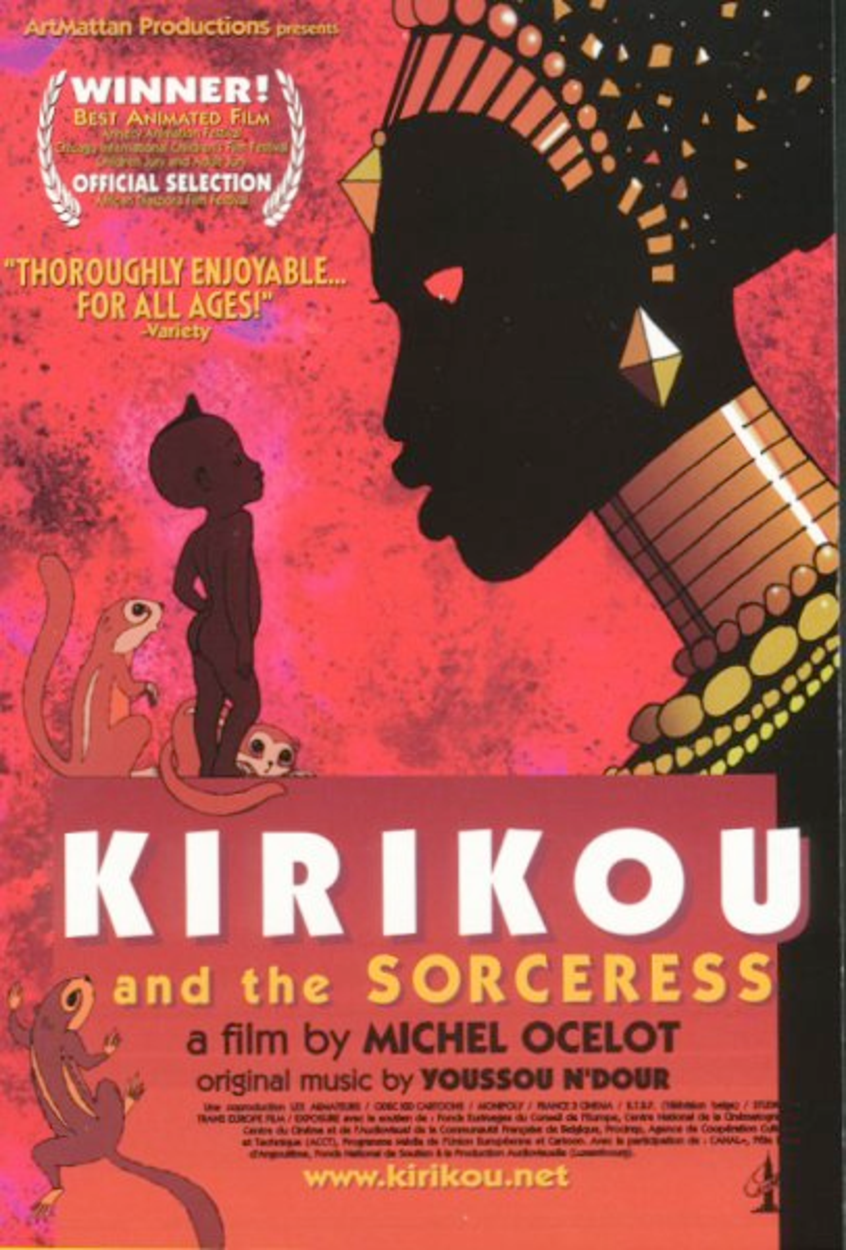
\includegraphics[width=\marginparwidth]{../figs/Kirikou}
\scriptsize{Kirikou and the sorceress, a film by Michel Ocelot with original music
by Youssou N'Dour.}
}. He is the main character of the animated film \textit{Kirikou et la sorci{\`e}re}
(Kirikou and the sorceress, 1998) and \textit{Kirikou et les b{\^e}tes sauvages}
(Kirikou and the Wild Beasts, 2005). Kirikou was chosen as a symbol of \seqinr{}
development time. \Seqinr{} started in september 2002 as part of the work of
Delphine Charif's master of sciences. The first public presentation of \seqinr{}
was a seminar (2-JUL-2003, Lausanne University, Swiss) and the first public
release on the CRAN\footnote{
Comprehensive R Archive Network.
} was in october 2004.

\section*{Technical details}

The cover was saved from Canvas into an EPS\footnote{
Encapsulated Postscrit.
} file. This file was then manually 
edited to remove non-ASCII characters. It was then converted into RGML\footnote{
RDF (Resource Description Framework) Graph Modeling Language (\url{http://www.cs.rpi.edu/~puninj/RGML/}).
} format
with the following \Rlogo{}~code based on \texttt{grid} \cite{grid},
\texttt{XML} \cite{XML} and \texttt{grImport} \cite{grImport}:
 
\begin{Schunk}
\begin{Sinput}
 library(grid)
 library(XML)
 library(grImport)
 PostScriptTrace("../figs/couverture.eps", "../figs/couverture.rgml")
\end{Sinput}
\end{Schunk}

The picture was then edited to add automatically 
the current \seqinr{}~release number:


\begin{Schunk}
\begin{Sinput}
 cover <- readPicture("../figs/couverture.rgml")
 pdf(file = "../figs/cover.pdf", width = 21/2.54, height = 29.7/2.54)
 pushViewport(plotViewport(margins = c(0, 0, 0, 0)))
 grid.picture(cover)
 grid.text(paste("SeqinR", packageDescription("seqinr")$Version), 
     gp = gpar(cex = 5), y = unit(0.72, "npc"))
 popViewport()
 dev.off()
\end{Sinput}
\end{Schunk}

And finally inserted at the begining of the \LaTeX~file with:

\begin{verbatim}
\atxy(0cm,0cm){
  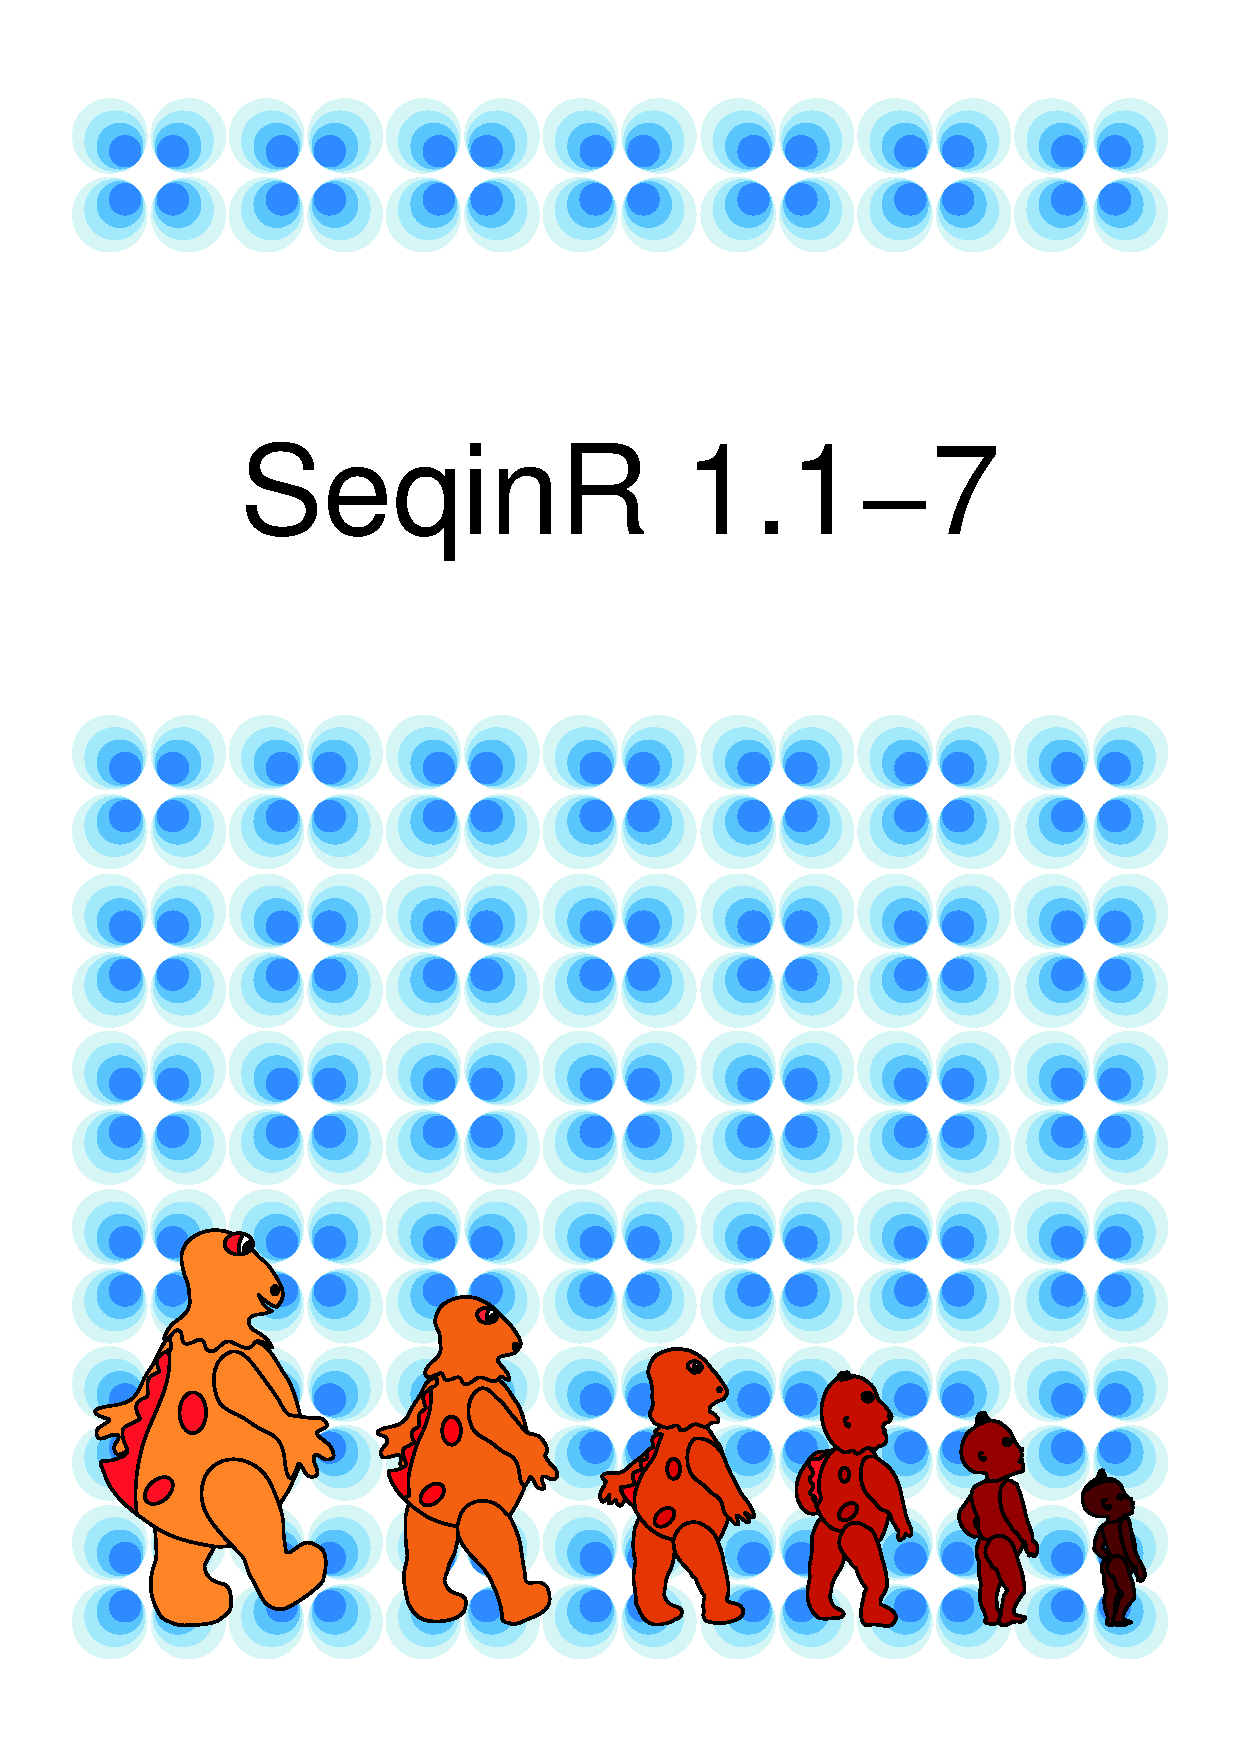
\includegraphics[width=\paperwidth,height=\paperheight]{../figs/cover}
}
\end{verbatim}



\section*{Session Informations}

This part was compiled under the following \Rlogo{}~environment:

\begin{itemize}
  \item R version 2.8.0 (2008-10-20), \verb|i386-apple-darwin8.8.2|
  \item Locale: \verb|fr_FR.UTF-8/fr_FR.UTF-8/fr_FR.UTF-8/C/C/C|
  \item Base packages: base, datasets, grDevices, graphics, grid,
    methods, stats, utils
  \item Other packages: MASS~7.2-44, XML~1.98-1, ade4~1.4-9,
    ape~2.2-2, grImport~0.3-1, nlme~3.1-89, quadprog~1.4-11,
    seqinr~2.0-1, tseries~0.10-16, xtable~1.5-4, zoo~1.5-4
  \item Loaded via a namespace (and not attached): lattice~0.17-15,
    tools~2.8.0
\end{itemize}
There were two compilation steps:

\begin{itemize}
  \item \Rlogo{} compilation time was: Fri Dec 12 14:54:35 2008
  \item \LaTeX{} compilation time was: \today
\end{itemize}


% END - DO NOT REMOVE THIS LINE

%%%%%%%%%%%%  BIBLIOGRAPHY %%%%%%%%%%%%%%%%%

\bibliographystyle{plain}
\bibliography{../config/book}
\end{document}
